\chapter{Planificación y Gestión del TFG}
\section{Planificación del Proyecto}
\subsection{Identificación de Interesados}
Se identifican los siguientes grupos de interesados en el proyecto:
\begin{itemize}
	\item Turistas: como usuarios finales de la aplicación, su satisfacción y experiencia de uso es fundamental para el éxito del proyecto.
	\item Empresa: como la empresa que solicita la aplicación, espera obtener un producto de alta calidad que cumpla con sus requisitos y expectativas.
	\item Desarrolladores: los encargados de construir y mantener la aplicación, quienes necesitan especificaciones claras y un entorno de desarrollo bien definido.
	\item Proveedores de Servicios Tecnológicos: empresas o entidades que proporcionan infraestructura tecnológica, como servidores, servicios en la nube, etc.
	\item Autoridades Reguladoras: organismos que supervisan el cumplimiento de las leyes y regulaciones pertinentes, como la LOPD, RGPD y LSSI-CE.
	\item Comunidad Local: residentes y negocios locales que podrían beneficiarse indirectamente del incremento del turismo y la mejora de servicios.
\end{itemize}
\subsection{OBS y PBS}
\subsubsection*{Organizational Breackdown Structure}
La ``Organizational Breackdown Structure`` (OBS) es una representación jerárquica de la estructura organizativa del proyecto.
Define los roles y responsabilidades de los miembros del equipo del proyecto y sus relaciones.
La OBS ayuda a comprender la estructura de informes, los canales de comunicación y la coordinación entre los diferentes interesados del proyecto.
\\[1ex]
En la siguiente figura, se representa la OBS utilizando un diagrama de bloques. Cada bloque representa un rol o posición específica dentro del equipo del proyecto. Las lineas indican las relaciones de informe entre los roles.

\begin{figure}[H]
	\centering
	\begin{adjustwidth}{-0.55cm}{}
		\begin{tikzpicture}[
				scale=0.7, every node/.style={scale=0.7},
				node distance = 3mm and 0mm,
				block/.style = {draw, rectangle, minimum height=20mm, text width=30mm, align=center, fill=gray!25},
				line/.style = {draw, thick}
			]

			% Nodos
			\node [block] (consultor) {Consultor de tecnología};
			\node [block, right=of consultor] (analista) {Analista};
			\node [block, right=of analista] (arquitecto) {Arquitecto de software};
			\node [block, right=of arquitecto] (desarrollador) {Desarrollador Full-Stack};
			\node [block, right=of desarrollador] (admin) {Administrador de base de datos};
			\node [block, right=of admin] (disenador) {Diseñador de UX/UI};
			\node [block, right=of disenador] (devops) {DevOps};
			\node [block, right=of devops] (tester) {Tester};
			\node [block, right=of desarrollador, yshift=30mm, xshift=-15mm] (director) {Director de proyecto};
			% Líneas
			\draw [line] ([yshift=2.5mm, xshift=16.5mm] desarrollador.north) -- ([yshift=10mm, xshift=16.5mm]desarrollador.north) ;
			\draw [line] ([yshift=2mm] consultor.north) -- ([yshift=2mm]tester.north) ;
			\draw [line] ([yshift=0mm] consultor.north) -- ([yshift=2mm]consultor.north) ;
			\draw [line] ([yshift=0mm] analista.north) -- ([yshift=2mm]analista.north) ;
			\draw [line] ([yshift=0mm] arquitecto.north) -- ([yshift=2mm]arquitecto.north) ;
			\draw [line] ([yshift=0mm] desarrollador.north) -- ([yshift=2mm]desarrollador.north) ;
			\draw [line] ([yshift=0mm] admin.north) -- ([yshift=2mm]admin.north) ;
			\draw [line] ([yshift=0mm] disenador.north) -- ([yshift=2mm]disenador.north) ;
			\draw [line] ([yshift=0mm] devops.north) -- ([yshift=2mm]devops.north) ;
			\draw [line] ([yshift=0mm] tester.north) -- ([yshift=2mm]tester.north) ;
		\end{tikzpicture}
	\end{adjustwidth}
	\caption{Organizational Breackdown Structure (OBS)}
\end{figure}

\subsubsection*{Product Breackdown Structure}
La ``Product Breackdown Structure`` (PBS) es una herramienta utilizada en la gestión de proyectos para descomponer el producto final en componentes más pequeños y manejables.
\\ [1ex]
La PBS facilita la planificación, estimación de costos, asignación de recursos y seguimiento del progreso del proyecto. Cada componente de la PBS representa una funcionalidad o característica específica del producto y puede descomponerse en más subcomponentes.
\\ [1ex]
En la siguiente figura, se representa la PBS utilizando un diagrama de bloques. Cada bloque representa una fase del proyecto y sus actividades asociadas. Las lineas indican la secuencia de las fases del proyecto.

\tikzset{
	base/.style = {draw, text width=30mm, minimum height=20mm, align=center},
	fase/.style = {base, fill=gray!30, rectangle},
	actividad/.style = {base, fill=gray!10},
	linea/.style = {draw, thick}
}

\begin{figure}[H]
	\centering
	\begin{adjustwidth}{-0.45cm}{}
		\begin{tikzpicture}[scale=0.7, every node/.style={scale=0.7}, node distance=3mm and 3mm]
			% Fases
			\node[fase] (gestion) {Gestión inicial};
			\node[fase, right=of gestion] (analisis) {Análisis};
			\node[fase, right=of analisis] (diseno) {Diseño};
			\node[fase, right=of diseno] (implementacion) {Implementación};
			\node[fase, right=of implementacion] (pruebas) {Pruebas};
			\node[fase, right=of pruebas] (documentacion) {Documentación};
			\node[fase, right=of documentacion] (cierre) {Cierre de proyecto};
			\node[fase, right=of diseno, yshift=25mm] (proyecto) {Proyecto};
			% ... Otras fases

			% Actividades de Gestión Inicial
			\node[actividad, below=of gestion, xshift=2.5mm] (explicacion) {Explicación del proyecto};
			\node[actividad, below=of explicacion] (estudio) {Estudio de las alternativas tecnológicas};
			%\node[actividad, below=of estudio] (viabilidad) {Estudio de la viabilidad};
			\node[actividad, below=of estudio] (planificacion) {Planificación del proyecto};
			\node[actividad, below=of planificacion] (creacion) {Creación de un plan de gestion de riesgos};
			\node[actividad, below=of creacion] (riesgos) {Identificación de riesgos};
			\node[actividad, below=of riesgos] (pinicial) {Realización del presupuesto inicial};
			% Actividades de Análisis
			\node[actividad, below=of analisis, xshift=2.5mm] (definicion) {Definición del alcance del sistema};
			\node[actividad, below=of definicion] (requisitos) {Análisis de los requisitos};
			\node[actividad, below=of requisitos] (acasos) {Análisis de los casos de uso};
			\node[actividad, below=of acasos] (aclases) {Análisis de las clases};
			\node[actividad, below=of aclases] (prototipos) {Diseño de los prototipos de las interfaces de usuario};
			\node[actividad, below=of prototipos] (plan) {Elaboración del plan de pruebas};
			% Actividades de Diseño
			\node[actividad, below=of diseno, xshift=2.5mm] (dcasos) {Diseño de casos de uso};
			\node[actividad, below=of dcasos] (dclases) {Diseño de clases};
			\node[actividad, below=of dclases] (darquitectura) {Diseño de la arquitectura del sistema};
			\node[actividad, below=of darquitectura] (mbbdd) {Modelado de bases de datos};
			\node[actividad, below=of mbbdd] (inter) {Diseño de la interfaz de usuario};
			\node[actividad, below=of inter] (dpruebas) {Diseño de pruebas};
			% Actividades de Implementación
			\node[actividad, below=of implementacion, xshift=2.5mm] (repo) {Creación de los repositorios};
			\node[actividad, below=of repo] (server) {Creación del servidor de aplicaciones};
			\node[actividad, below=of server] (cliente) {Creación de la aplicación del cliente};
			\node[actividad, below=of cliente] (intebbdd) {Integración de la base de datos};
			\node[actividad, below=of intebbdd] (gusuarios) {Implementación del subsistema de gestión de usuarios};
			\node[actividad, below=of gusuarios] (gactividades) {Implementación del subsistema de gestión de actividades};
			\node[actividad, below=of gactividades] (greservas) {Implementación del subsistema de gestión de reservas};
			\node[actividad, below=of greservas] (pasarela) {Integración de la pasarela de pago};
			\node[actividad, below=of pasarela] (codeinter) {Codificación de estilos e interfaz de usuario};
			% Actividades de Pruebas
			\node[actividad, below=of pruebas, xshift=2.5mm] (uni) {Desarrollo de pruebas unitarias};
			\node[actividad, below=of uni] (inte) {Desarrollo de pruebas de integración};
			\node[actividad, below=of inte] (acces) {Desarrollo de pruebas de accesibilidad};

			%Documentación
			\node[actividad, below=of documentacion, xshift=2.5mm] (instalacion) {Manual de instalación};
			\node[actividad, below=of instalacion] (ejecucion) {Manual de ejecución};
			\node[actividad, below=of ejecucion] (musuario) {manual de usuario};

			%Cierre
			\node[actividad, below=of cierre, xshift=2.5mm] (planicierre) {Elaboración de la planificacion de cierre};
			\node[actividad, below=of planicierre] (preucierre) {Calculo del presupuesto final};
			\node[actividad, below=of preucierre] (reucierre) {Reunion de cierre};


			% Conexiones entre fases
			\draw[linea] ([yshift=2.5mm]gestion.north) -- ([yshift=2.5mm]cierre.north);
			\draw[linea] (gestion.north) -- +(0,3mm);
			\draw[linea] (analisis.north) -- +(0,3mm);
			\draw[linea] (diseno.north) -- +(0,3mm);
			\draw[linea] (implementacion.north) -- +(0,5mm);
			\draw[linea] (pruebas.north) -- +(0,3mm);
			\draw[linea] (documentacion.north) -- +(0,3mm);
			\draw[linea] (cierre.north) -- +(0,3mm);

			% Conexiones entre actividades
			\draw[linea] ([xshift=-16mm]gestion.south) -- ([xshift=-18.5mm,yshift=10mm]pinicial.south);
			\draw[linea] (explicacion.west) -- +(-2mm,0);
			\draw[linea] (estudio.west) -- +(-2mm,0);
			\draw[linea] (planificacion.west) -- +(-2mm,0);
			\draw[linea] (creacion.west) -- +(-2mm,0);
			\draw[linea] (riesgos.west) -- +(-2mm,0);
			\draw[linea] (pinicial.west) -- +(-2mm,0);

			\draw[linea] ([xshift=-16mm]analisis.south) -- ([xshift=-18.5mm,yshift=10mm]plan.south);
			\draw[linea] (definicion.west) -- +(-2mm,0);
			\draw[linea] (requisitos.west) -- +(-2mm,0);
			\draw[linea] (acasos.west) -- +(-2mm,0);
			\draw[linea] (aclases.west) -- +(-2mm,0);
			\draw[linea] (prototipos.west) -- +(-2mm,0);
			\draw[linea] (plan.west) -- +(-2mm,0);

			\draw[linea] ([xshift=-16mm]diseno.south) -- ([xshift=-18.5mm,yshift=10mm]dpruebas.south);
			\draw[linea] (dcasos.west) -- +(-2mm,0);
			\draw[linea] (dclases.west) -- +(-2mm,0);
			\draw[linea] (darquitectura.west) -- +(-2mm,0);
			\draw[linea] (mbbdd.west) -- +(-2mm,0);
			\draw[linea] (inter.west) -- +(-2mm,0);
			\draw[linea] (dpruebas.west) -- +(-2mm,0);

			\draw[linea] ([xshift=-16mm]implementacion.south) -- ([xshift=-18.5mm,yshift=10mm]codeinter.south);
			\draw[linea] (repo.west) -- +(-2mm,0);
			\draw[linea] (server.west) -- +(-2mm,0);
			\draw[linea] (cliente.west) -- +(-2mm,0);
			\draw[linea] (intebbdd.west) -- +(-2mm,0);
			\draw[linea] (gusuarios.west) -- +(-2mm,0);
			\draw[linea] (gactividades.west) -- +(-2mm,0);
			\draw[linea] (greservas.west) -- +(-2mm,0);
			\draw[linea] (pasarela.west) -- +(-2mm,0);
			\draw[linea] (codeinter.west) -- +(-2mm,0);

			\draw[linea] ([xshift=-16mm]pruebas.south) -- ([xshift=-18.5mm,yshift=10mm]acces.south);
			\draw[linea] (uni.west) -- +(-2mm,0);
			\draw[linea] (inte.west) -- +(-2mm,0);
			\draw[linea] (acces.west) -- +(-2mm,0);

			\draw[linea] ([xshift=-16mm]documentacion.south) -- ([xshift=-18.5mm,yshift=10mm]musuario.south);
			\draw[linea] (instalacion.west) -- +(-2mm,0);
			\draw[linea] (ejecucion.west) -- +(-2mm,0);
			\draw[linea] (musuario.west) -- +(-2mm,0);

			\draw[linea] ([xshift=-16mm]cierre.south) -- ([xshift=-18.5mm,yshift=10mm]reucierre.south);
			\draw[linea] (planicierre.west) -- +(-2mm,0);
			\draw[linea] (preucierre.west) -- +(-2mm,0);
			\draw[linea] (reucierre.west) -- +(-2mm,0);

		\end{tikzpicture}
	\end{adjustwidth}
	\caption{Product Breackdown Structure}
\end{figure}

\subsection{Planificación Inicial. WBS}
Se estima que se emplearán 640 horas para elaborar el proyecto, comenzando el día 1 de marzo de 2023 y finalizando el día 31 de mayo de 2023. Se trabajarían 49 horas semanales, es decir, 7 horas al día de lunes a domingo.\\[1ex]
La planificación se ha dividido en varias fases:
\begin{planificacion}
	\centering
	\begin{tabular}{ | m{9cm} | c | c | c |}
		\hline
		\textbf{Fase}      & \textbf{Duración (horas)} & \textbf{Comienzo} & \textbf{Fin} \\
		\hline
		Gestión inicial    & 63                        & 1/3/23            & 9/3/23       \\
		\hline
		Análisis           & 56                        & 10/3/23           & 17/3/23      \\
		\hline
		Diseño             & 113                       & 18/3/23           & 3/4/23       \\
		\hline
		Implementación     & 287                       & 3/4/23            & 14/5/23      \\
		\hline
		Pruebas            & 105                       & 14/5/23           & 29/5/23      \\
		\hline
		Documentación      & 11                        & 29/5/23           & 30/5/23      \\
		\hline
		Cierre de proyecto & 5                         & 30/5/23           & 31/5/23      \\
		\hline
	\end{tabular}
	\caption{Resumen de Fases y Cronograma del Proyecto}
\end{planificacion}

\subsubsection{Gestión inicial}
\begin{planificacion}
	\centering
	\begin{tabular}{ | m{9cm} | c | c | c |}
		\hline
		\textbf{Nombre de tarea}                  & \textbf{Duración (horas)} & \textbf{Comienzo} & \textbf{Fin} \\
		\hline
		Explicación del proyecto                  & 2                         & 1/3/23            & 1/3/23       \\
		\hline
		Estudio de las alternativas tecnológicas  & 10                        & 1/3/23            & 2/3/23       \\
		\hline
		Selección de la arquitectura tecnológica  & 5                         & 2/3/23            & 3/3/23       \\
		\hline
		Estudio de viabilidad                     & 15                        & 3/3/23            & 5/3/23       \\
		\hline
		Planificación del proyecto                & 10                        & 5/3/23            & 6/3/23       \\
		\hline
		Creación de un plan de gestión de riesgos & 8                         & 7/3/23            & 8/3/23       \\
		\hline
		Identificación de riesgos                 & 8                         & 8/3/23            & 9/3/23       \\
		\hline
		Realización del presupuesto inicial       & 5                         & 9/3/23            & 9/3/23       \\
		\hline
	\end{tabular}
	\caption{Detalle de Tareas y Cronograma de la Fase de Gestión Inicial}
\end{planificacion}

\subsubsection{Análisis}
\begin{planificacion}
	\centering
	\begin{tabular}{ | m{9cm} | c | c | c | }
		\hline
		\textbf{Nombre de la tarea}                           & \textbf{Duración (horas)} & \textbf{Comienzo} & \textbf{Fin} \\\hline
		Definición del alcance del sistema                    & 5                         & 10/3/23           & 10/3/23      \\\hline
		Análisis de los requisitos                            & 15                        & 10/3/23           & 12/3/23      \\\hline
		Análisis de los casos de uso                          & 15                        & 12/3/23           & 14/3/23      \\\hline
		Análisis de clases                                    & 8                         & 15/3/23           & 16/3/23      \\\hline
		Diseño de los prototipos de las interfaces de usuario & 5                         & 16/3/23           & 16/3/23      \\\hline
		Elaboración del plan de pruebas                       & 8                         & 16/3/23           & 17/3/23      \\\hline
	\end{tabular}
	\caption{Detalle de Tareas y Cronograma de la Fase de Análisis}
	\label{table:analysis_design_phase}
\end{planificacion}
\subsubsection{Diseño}
\input{4-PlanificacionYGestionDelTFG/PlanificacionInicial/TablaDiseño}
\subsubsection{Implementación}
\begin{planificacion}
	\centering
	\begin{tabular}{ | m{9cm} | c | c | c |}
		\hline
		\textbf{Nombre de la tarea}                             & \textbf{Duración (horas)} & \textbf{Comienzo} & \textbf{Fin} \\
		\hline
		Creación de los repositorios                            & 2                         & 3/4/23            & 3/4/23       \\
		\hline
		Creación del servidor de aplicaciones                   & 2                         & 3/4/23            & 3/4/23       \\
		\hline
		Creación de la aplicación cliente                       & 2                         & 3/4/23            & 3/4/23       \\
		\hline
		Integración de la base de datos                         & 5                         & 4/4/23            & 4/4/23       \\
		\hline
		Implementación del subsistema de gestión de usuarios    & 20                        & 4/4/23            & 7/4/23       \\
		\hline
		Implementación del subsistema de gestión de actividades & 30                        & 7/4/23            & 11/4/23      \\
		\hline
		Implementación del subsistema de gestión de reservas    & 100                       & 11/4/23           & 26/4/23      \\
		\hline
		Integración de pasarela de pago                         & 50                        & 26/4/23           & 3/5/23       \\
		\hline
		Codificación de estilos e interfaz de usuario           & 50                        & 3/5/23            & 10/5/23      \\
		\hline
		Despliegue del entorno                                  & 26                        & 10/5/23           & 14/5/23      \\
		\hline
	\end{tabular}
	\caption{Detalle de Tareas y Cronograma de la Fase de Implementación}
\end{planificacion}
\subsubsection{Pruebas}
\begin{planificacion}
	\centering
	\begin{tabular}{ | m{9cm} | c | c | c |}
		\hline
		\textbf{Nombre de la tarea}          & \textbf{Duración (horas)} & \textbf{Comienzo} & \textbf{Fin} \\
		\hline
		Desarrollo de pruebas unitarias      & 50                        & 14/5/23           & 21/5/23      \\
		\hline
		Desarrollo de pruebas de integración & 40                        & 21/5/23           & 26/5/23      \\
		\hline
		Desarrollo de pruebas de usabilidad  & 15                        & 27/5/23           & 29/5/23      \\
		\hline
	\end{tabular}
	\caption{Detalle de Tareas y Cronograma de la Fase de Pruebas}
\end{planificacion}

\subsubsection{Documentación}
\begin{planificacion}
	\centering
	\begin{tabular}{ | m{9cm} | c | c | c | }
		\hline
		\textbf{Nombre de la tarea} & \textbf{Duración (horas)} & \textbf{Comienzo} & \textbf{Fin} \\\hline
		Manual de instalación       & 2                         & 29/5/23           & 29/5/23      \\\hline
		Manual de ejecución         & 1                         & 29/5/23           & 30/5/23      \\\hline
		Manual de usuario           & 8                         & 29/5/23           & 30/5/23      \\\hline
	\end{tabular}
	\caption{Detalle de Tareas y Cronograma de la Fase de Documentación}
\end{planificacion}

\subsubsection{Cierre de Proyecto}
\begin{planificacion}
	\centering
	\begin{tabular}{ | m{9cm} | c | c | c | }
		\hline
		\textbf{Nombre de la tarea}           & \textbf{Duración (horas)} & \textbf{Comienzo} & \textbf{Fin} \\\hline
		Elaboración de la planificación final & 2                         & 30/5/23           & 30/5/23      \\\hline
		Cálculo del presupuesto final         & 2                         & 31/5/23           & 31/5/23      \\\hline
		Reunión de cierre del proyecto        & 1                         & 31/5/23           & 31/5/23      \\\hline
	\end{tabular}
	\caption{Detalle de Tareas y Cronograma de la Fase de Cierre del Proyecto}
\end{planificacion}

\subsubsection{Diagrama de Gantt}

\begin{figure}[H]
	\centering
	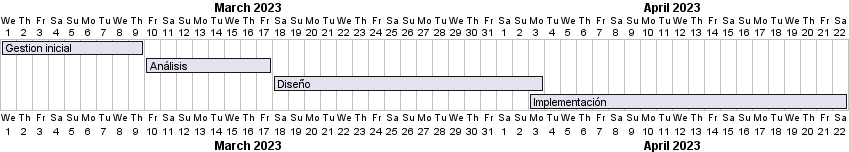
\includegraphics[width=1\textwidth]{4-PlanificacionYGestionDelTFG/PlanificacionInicial/gant1.png}
	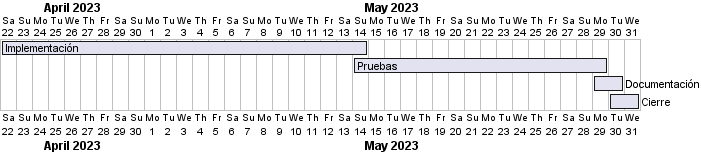
\includegraphics[width=0.8\textwidth]{4-PlanificacionYGestionDelTFG/PlanificacionInicial/gant2.png}
	\caption{Diagrama de Gantt de la planificación inicial del proyecto}
\end{figure}

\begin{figure}[H]
	\centering
	\begin{minipage}{0.45\textwidth}
		\includegraphics[width=1\textwidth]{4-PlanificacionYGestionDelTFG/PlanificacionInicial/gant-gestionInicial.png}
		\caption{Diagrama de Gantt de la fase de gestión inicial}
	\end{minipage}
	\hfill
	\begin{minipage}{0.45\textwidth}
		\centering
		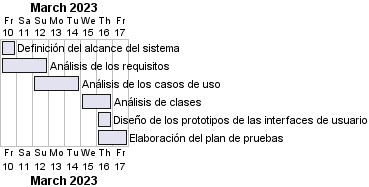
\includegraphics[width=1\textwidth]{4-PlanificacionYGestionDelTFG/PlanificacionInicial/gant-analisis.png}
		\caption{Diagrama de Gantt de la fase de análisis}
	\end{minipage}
\end{figure}

\begin{figure}[H]
	\centering
	\includegraphics[width=0.6\textwidth]{4-PlanificacionYGestionDelTFG/PlanificacionInicial/gant-diseño.png}
	\caption{Diagrama de Gantt de la fase de diseño}
\end{figure}

\begin{figure}[H]
	\centering
	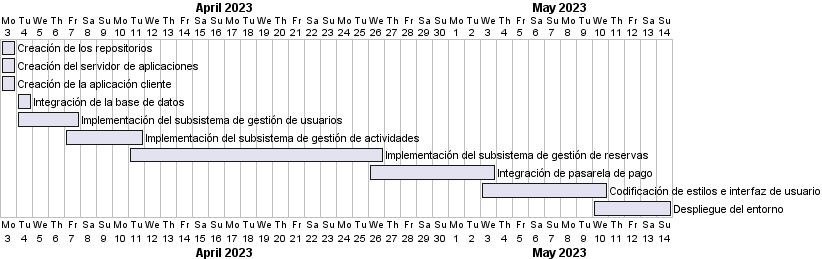
\includegraphics[width=1\textwidth]{4-PlanificacionYGestionDelTFG/PlanificacionInicial/gant-implementacion.png}
	\caption{Diagrama de Gantt de la fase de implementación}
\end{figure}

\begin{figure}[H]
	\centering
	\begin{minipage}{0.65\textwidth}
		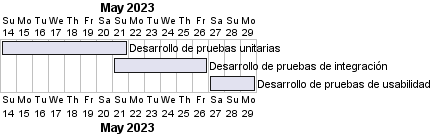
\includegraphics[width=1\textwidth]{4-PlanificacionYGestionDelTFG/PlanificacionInicial/gant-pruebas.png}
		\caption{Diagrama de Gantt de la fase de pruebas}
	\end{minipage}
	\hfill
	\begin{minipage}{0.25\textwidth}
		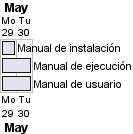
\includegraphics[width=1\textwidth]{4-PlanificacionYGestionDelTFG/PlanificacionInicial/gant-documentacion.png}
		\caption{Diagrama de Gantt de la fase de documentación}
	\end{minipage}
\end{figure}

\begin{figure}[H]
	\centering
	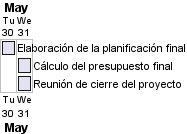
\includegraphics[width=0.4\textwidth]{4-PlanificacionYGestionDelTFG/PlanificacionInicial/gant-cierre.png}
	\caption{Diagrama de Gantt de la fase de cierre de proyecto}
\end{figure}
\subsection{Riesgos}
\subsubsection{Plan de Gestión de Riesgos}
El contenido del plan de gestión de riesgos se desarrolla en el \textit{Apéndice \ref{appendix:plan-gestion-riesgos}. Plan de gestión de riesgos}.
\subsubsection{Identificación de Riesgos}
\begin{table}[H]
	\centering
	\begin{tabular}{|c|m{4cm}|m{10cm}|}
		\hline
		{\textbf{ID}} & {\textbf{Nombre del riesgo}} & {\textbf{Descripción}}                                                                                                                                               \\
		\hline
		R1            & Problemas de compatibilidad  & Puede haber problemas de compatibilidad con las diferentes versiones de los navegadores o dispositivos móviles                                                       \\
		\hline
		R2            & Cambios de requisitos        & Puede haber una escasez de recursos como presupuesto, tiempo y equipos de desarrollo adecuados, lo que puede afectar la calidad y la eficiencia del proyecto         \\
		\hline
		R3            & Problemas de seguridad       & La aplicación puede estar expuesta a vulnerabilidades de seguridad que pueden ser explotadas por atacantes malintencionados.                                         \\
		\hline
		R4            & Falta de pruebas adecuadas   & La falta de pruebas adecuadas puede llevar a la liberación de una aplicación con errores y problemas de rendimientos.                                                \\
		\hline
		R5            & Problemas de rendimiento     & La aplicación puede ser lenta o ineficiente debido a problemas de diseño o codificación.                                                                             \\
		\hline
		R6            & Fallos de integración        & Puede haber problemas al integrar diferentes componentes y sistemas de la aplicación.                                                                                \\
		\hline
		R7            & Falta de experiencia         & La falta de experiencia en el equipo de desarrollo puede afectar la calidad del código y la capacidad para resolver problemas complejos.                             \\
		\hline
		R8            & Errores de estimación        & Puede haber errores de estimación en cuanto a la duración y los recursos necesarios para completar el proyecto que pueden afectar la planificación y el presupuesto. \\
		\hline
		R9            & Problemas de comunicación    & La falta de comunicación o una mala comunicación entre los miembros del equipo o con los clientes puede llevar a malentendidos y errores.                            \\
		\hline
		R10           & Problemas de calidad         & Puede haber problemas de calidad en el código, la documentación o los procesos de desarrollo que pueden afectar la fiabilidad y la estabilidad de la aplicación.     \\
		\hline
	\end{tabular}
	\caption{Tabla de riesgos identificados}
\end{table}
\subsubsection{Registro de Riesgos}
Se incluirán los riesgos detallados en el \textit{Apéndice \ref{appendix:hojas-riesgos}. Hojas de riesgos}. Especificando tanto su impacto como su probabilidad.
\subsection{Presupuesto Inicial}
En esta sección se presentan las tarifas por hora estimadas para cada perfil profesional que se utilizarán para calcular los costos del proyecto.
Los precios por hora se han calculado tomando como referencia los salarios base anuales de cada perfil, de acuerdo con datos del mercado actual \cite{manfred2023}.
\begin{planificacion}
	\centering
	\begin{tabular}{ | m{9cm} | c | }
		\hline
		\textbf{Perfil}                & \textbf{Precio/hora} \\\hline
		Consultor de tecnología        & 35,55€               \\\hline
		Analista                       & 31,72€               \\\hline
		Arquitecto de software         & 36,65€               \\\hline
		Desarrollador Full-Stack       & 21,88€               \\\hline
		Arquitecto de software         & 27,30€               \\\hline
		Administrador de base de datos & 31,72€               \\\hline
		Diseñador de UX/UI             & 25,71€               \\\hline
		DevOps                         & 21,88€               \\\hline
		Tester                         & 16,41€               \\\hline
		Director de proyecto           & 33,91€               \\\hline
	\end{tabular}
	\caption{Presupuesto por perfil profesional}
\end{planificacion}

Los datos de las tarifas por hora han sido calculados a partir de los salarios base anuales de cada perfil.
A continuación, se detalla la referencia salarial utilizada para cada perfil:
\begin{itemize}
	\item  \textbf{Desarrollador Full-Stack:} 40.000€ anuales.
	\item  \textbf{Arquitecto de software:} 67.000€ anuales.
	\item  \textbf{Diseñador de UX/UI:} 47.000€ anuales.
	\item  \textbf{Tester:} 30.000€ anuales.
	\item  \textbf{Administrador de base de datos:} 58.000€ anuales.
	\item  \textbf{Analista:} 58.000€ anuales.
	\item  \textbf{Director de proyecto:} 62.000€ anuales.
	\item  \textbf{DevOps:} 40.000€ anuales.
	\item  \textbf{Consultor de tecnología:} 65.000€ anuales.
\end{itemize}
El precio por hora se ha calculado considerando una jornada laboral anual de 1.828 horas.
\subsubsection{Presupuesto de costes}
Para una mejor planificación y control del presupuesto del proyecto, se ha dividido el coste en varias fases.
Cada fase del proyecto representa un conjunto de actividades y entregables específicos.
A continuación, se presenta un desglose detallado de los costes asociados a cada fase del proyecto.
\\[1ex]
Este desglose permite identificar de manera clara y precisa los recursos necesarios y los costes estimados en cada etapa, facilitando así la gestión y asignación de los recursos a lo largo del ciclo de vida del proyecto.
\begin{planificacion}
	\centering
	\begin{tabular}{ | m{8.5cm} | c | m{2.5cm} |  m{1.5cm} |}
		\hline
		\textbf{Nombre de tarea}                  & \textbf{Duración(horas)} & \textbf{Perfil}         & \textbf{Precio} \\\hline
		Explicación del proyecto                  & 2                        & Director de proyecto    & 67,82€          \\\hline
		Estudio de las alternativas tecnológicas  & 10                       & Consultor de tecnología & 355,50€         \\\hline
		Selección de la arquitectura tecnológica  & 5                        & Arquitecto de software  & 183,25€         \\\hline
		Estudio de viabilidad                     & 15                       & Analista                & 475,80€         \\\hline
		Planificación del proyecto                & 10                       & Director de proyecto    & 339,10€         \\\hline
		Creación de un plan de gestión de riesgos & 8                        & Consultor de tecnología & 284,40€         \\\hline
		Identificación de riesgos                 & 8                        & Consultor de tecnología & 284,40€         \\\hline
	\end{tabular}
	\caption{Presupuesto inicial de la fase de gestión inicial}
\end{planificacion}

\begin{planificacion}
	\centering
	\begin{tabular}{ | m{8.5cm} | c | m{2.5cm} |  m{1.5cm} |}
		\hline
		\textbf{Nombre de la tarea}                           & \textbf{Duración(horas)} & \textbf{Perfil}    & \textbf{Precio} \\\hline
		Definición del alcance del sistema                    & 5                        & Analista           & 158,60€         \\\hline
		Análisis de los requisitos                            & 15                       & Analista           & 475,80€         \\\hline
		Análisis de los casos de uso                          & 15                       & Analista           & 475,80€         \\\hline
		Análisis de clases                                    & 8                        & Analista           & 253,76€         \\\hline
		Diseño de los prototipos de las interfaces de usuario & 5                        & Diseñador de UX/UI & 128,55€         \\\hline
		Elaboración del plan de pruebas                       & 8                        & Tester             & 131,28€         \\\hline
	\end{tabular}
	\caption{Presupuesto inicial de la fase de análisis}
\end{planificacion}

\begin{planificacion}
	\centering
	\begin{tabular}{ | m{8.5cm} | c | m{2.5cm} |  m{1.5cm} |}
		\hline
		\textbf{Nombre de la tarea}                      & \textbf{Duración(horas)} & \textbf{Perfil}                & \textbf{Precio} \\\hline
		Diseño de casos de uso reales                    & 15                       & Arquitecto de software         & 549,75€         \\\hline
		Diseño de clases                                 & 10                       & Arquitecto de software         & 366,50€         \\\hline
		Diseño de la arquitectura de módulos del sistema & 8                        & Arquitecto de software         & 293,20€         \\\hline
		Modelado de bases de datos                       & 5                        & Administrador de base de datos & 158,60€         \\\hline
		Diseño de la interfaz de usuario                 & 50                       & Diseñador de UX/UI             & 1285,50€        \\\hline
		Diseño de pruebas                                & 25                       & Tester                         & 410,25€         \\\hline
	\end{tabular}
	\caption{Presupuesto inicial de la fase de diseño}
\end{planificacion}

\begin{planificacion}
	\centering
	\begin{tabular}{ | m{8.5cm} | c | m{2.5cm} |  m{1.5cm} |}
		\hline
		\textbf{Nombre de la tarea}                             & \textbf{Duración(horas)} & \textbf{Perfil}                & \textbf{Precio} \\\hline
		Creación de los repositorios                            & 2                        & DevOps                         & 43,76€          \\\hline
		Creación del servidor de aplicaciones                   & 2                        & DevOps                         & 43,76€          \\\hline
		Creación de la aplicación cliente                       & 2                        & Desarrollador Full-Stack       & 43,76€          \\\hline
		Integración de la base de datos                         & 5                        & Administrador de base de datos & 158,60€         \\\hline
		Implementación del subsistema de gestión de usuarios    & 20                       & Desarrollador Full-Stack       & 437,60€         \\\hline
		Implementación del subsistema de gestión de actividades & 30                       & Desarrollador Full-Stack       & 656,40€         \\\hline
		Implementación del subsistema de gestión de reservas    & 100                      & Desarrollador Full-Stack       & 2188,00€        \\\hline
		Integración de pasarela de pago                         & 50                       & Desarrollador Full-Stack       & 1094,00€        \\\hline
		Codificación de estilos e interfaz de usuario           & 50                       & Diseñador de UX/UI             & 1285,50€        \\\hline
		Despliegue del entorno                                  & 26                       & DevOps                         & 568,88€         \\\hline
	\end{tabular}
	\caption{Presupuesto inicial de la fase de implementación}
\end{planificacion}

\begin{planificacion}
	\centering
	\begin{tabular}{ | m{8.5cm} | c | m{2.5cm} |  m{1.5cm} |}
		\hline
		\textbf{Nombre de la tarea}          & \textbf{Duración(horas)} & \textbf{Perfil} & \textbf{Precio} \\\hline
		Desarrollo de pruebas unitarias      & 50                       & Tester          & 820,50€         \\\hline
		Desarrollo de pruebas de integración & 40                       & Tester          & 656,40€         \\\hline
		Desarrollo de pruebas de usabilidad  & 15                       & Tester          & 246,15€         \\\hline
	\end{tabular}
	\caption{Presupuesto inicial de la fase de pruebas}
\end{planificacion}

\begin{planificacion}
	\centering
	\begin{tabular}{ | m{8.5cm} | c | m{2.5cm} |  m{1.5cm} |}
		\hline
		\textbf{Nombre de la tarea} & \textbf{Duración(horas)} & \textbf{Perfil}          & \textbf{Precio} \\\hline
		Manual de instalación       & 2                        & Desarrollador Full-Stack & 43,76€          \\\hline
		Manual de ejecución         & 1                        & Desarrollador Full-Stack & 21,88€          \\\hline
		Manual de usuario           & 8                        & Diseñador de UX/UI       & 205,68€         \\\hline
	\end{tabular}
	\caption{Presupuesto inicial de la fase de documentación}
\end{planificacion}

\begin{planificacion}
	\centering
	\begin{tabular}{ | m{8.5cm} | c | m{2.5cm} |  m{1.5cm} |}
		\hline
		\textbf{Nombre de la tarea}           & \textbf{Duración(horas)} & \textbf{Perfil}      & \textbf{Precio} \\\hline
		Elaboración de la planificación final & 2                        & Director de proyecto & 67,82€          \\\hline
		Cálculo del presupuesto final         & 2                        & Director de proyecto & 67,82€          \\\hline
		Reunión de cierre del proyecto        & 1                        & Director de proyecto & 33,91€          \\\hline
	\end{tabular}
	\caption{Presupuesto inicial de la fase de cierre de proyecto}
\end{planificacion}
\subsubsection{Presupuesto total de costes}
En esta sección se presenta una visión global del presupuesto total del proyecto, sumando los costes desglosados por fases y perfiles profesionales.
El objetivo es proporcionar una estimación completa y detallada de los recursos financieros necesarios para llevar a cabo el proyecto de principio a fin.

\begin{planificacion}
	\centering
	\begin{tabular}{ | m{9cm} | c | c |}
		\hline
		\textbf{Fase}      & \textbf{Duración (horas)} & \textbf{Precio}    \\\hline
		Gestión inicial    & 63                        & 2148,87€           \\\hline
		Análisis           & 56                        & 1623,79€           \\\hline
		Diseño             & 113                       & 3063,85€           \\\hline
		Implementación     & 287                       & 6410,00€           \\\hline
		Pruebas            & 105                       & 1722,45€           \\\hline
		Documentación      & 11                        & 271,32€            \\\hline
		Cierre de proyecto & 5                         & 169,55€            \\\hline
		\textbf{Total}     & \textbf{640}              & \textbf{15809,83€} \\\hline
	\end{tabular}
	\caption{Presupuesto de costes total}
\end{planificacion}

\subsubsection{Presupuesto de cliente}
Se ha seleccionado un margen del 20\% de beneficio basándonos en un análisis exhaustivo de los costos y las prácticas estándar de la industria.
Este margen permite cubrir adecuadamente los costos directos e indirectos, así como los riesgos asociados al desarrollo del proyecto, como posibles retrasos y cambios en los requisitos.
\\[1ex]
Además, al mantener un margen del 20\%, podemos ofrecer un precio competitivo que añade valor al cliente, asegurando la viabilidad financiera y la sostenibilidad a largo plazo del proyecto sin imponer un costo excesivo.
Este equilibrio entre rentabilidad y accesibilidad es esencial para fomentar la confianza del cliente y apoyar el crecimiento futuro de la empresa.

\begin{planificacion}
	\centering
	\begin{tabular}{ | m{9cm} | c | c |}
		\hline
		\textbf{Fase}      & \textbf{Duración (horas)} & \textbf{Precio }   \\\hline
		Gestión inicial    & 63                        & 2578,64€           \\\hline
		Análisis           & 56                        & 1948,55€           \\\hline
		Diseño             & 113                       & 3676,62€           \\\hline
		Implementación     & 287                       & 7692,00€           \\\hline
		Pruebas            & 105                       & 2066,94€           \\\hline
		Documentación      & 11                        & 325,58€            \\\hline
		Cierre de proyecto & 5                         & 203,46€            \\\hline
		\textbf{Total}     & \textbf{640}              & \textbf{18991,79€} \\\hline
	\end{tabular}
	\caption{Presupuesto para el cliente}
\end{planificacion}


\section{Ejecución del proyecto}
\subsection{Bitácora de incidencias}
Se ha llevado un registro de las incidencias que han surgido durante el desarrollo del proyecto, así como su impacto en la planificación del mismo. A continuación, se muestra una tabla con las incidencias registradas y su efecto en la planificación del proyecto.
\begin{table}[H]
	\centering
	\begin{tabular}{ | c |  c | c | m{4.7cm} | m{4.3cm} | }
		\hline
		\textbf{ID} & \textbf{Fecha de creación} & \textbf{Fecha de cierre} & \textbf{Descripción de la incidencia}                                                          & \textbf{Efecto en la planificación}                                     \\
		\hline
		1           & 10/3/23                    & 13/6/23                  & Cambio del jefe de proyecto                                                                    & Retraso de 3 meses en la revisión de la planificación del proyecto      \\
		\hline
		2           & 1/7/23                     & 3/6/24                   & Asignación de un proyecto adicional al equipo, requiriendo redistribución de recursos y tiempo & Reducción de la jornada de trabajo de 7 horas a 2 horas y media diarias \\
		\hline
		3           & 27/9/23                    & 16/10/23                 & Problema con la subida de imágenes al servidor                                                 & Retraso de 49 horas en la implementación del subsistema de actividades  \\
		\hline
		4           & 25/3/24                    & 29/3/24                  & Problemas en el despliegue del servidor con AWS y Docker durante la fase de implementación     & Retraso de 10 horas en la puesta en marcha del entorno de despliegue    \\
		\hline
	\end{tabular}
	\caption{Registro de Incidencias y su Impacto en la Planificación del Proyecto}
\end{table}

\subsection{Riesgos}
A continuación, se presentan los riesgos identificados en la planificación del proyecto, así como su seguimiento a lo largo del desarrollo del mismo. Para cada riesgo se proporciona una descripción, el retraso causado y el evento de bitácora asociado.
\begin{table}[H]
	\centering
	\begin{tabular}{ | c | m{13cm} | }
		\hline
		{\textbf{R9}}               & {Problemas de comunicación}                                                                                         \\
		\hline
		\textbf{Descripción}        & Cambio del jefe de proyecto, lo que causó un retraso significativo en la revisión de la planificación del proyecto. \\
		\hline
		\textbf{Retraso}            & 3 meses                                                                                                             \\
		\hline
		\textbf{Evento de bitácora} & 1                                                                                                                   \\
		\hline
	\end{tabular}
	\caption{Seguimiento del riesgo de cambio del jefe de proyecto}
\end{table}

\vspace{0.5cm}

\begin{table}[H]
	\centering
	\begin{tabular}{ | c | m{13cm} | }
		\hline
		{\textbf{R8}}               & {Errores de estimación}                                                                                                                                                   \\
		\hline
		\textbf{Descripción}        & Asignación de un proyecto adicional al equipo, requiriendo una redistribución significativa de recursos y tiempo. Esto resultó en una reducción de la jornada de trabajo. \\
		\hline
		\textbf{Retraso}            & Reducción de la jornada de trabajo de 7 horas a 2 horas y media diarias                                                                                                   \\
		\hline
		\textbf{Evento de bitácora} & 2                                                                                                                                                                         \\
		\hline
	\end{tabular}
	\caption{Seguimiento del riesgo de redistribución de recursos y tiempo}
\end{table}

\vspace{0.5cm}

\begin{table}[H]
	\centering
	\begin{tabular}{ | c | m{13cm} | }
		\hline
		{\textbf{R6}}               & {Fallos de integración}                                                                                    \\
		\hline
		\textbf{Descripción}        & Problema con la subida de imágenes al servidor, afectando la implementación del subsistema de actividades. \\
		\hline
		\textbf{Retraso}            & 49 horas                                                                                                   \\
		\hline
		\textbf{Evento de bitácora} & 3                                                                                                          \\
		\hline
	\end{tabular}
	\caption{Seguimiento del riesgo de problemas de integración}
\end{table}

\vspace{0.5cm}

\begin{table}[H]
	\centering
	\begin{tabular}{ | c | m{13cm} | }
		\hline
		{\textbf{R7}}               & {Falta de experiencia}                                                                      \\
		\hline
		\textbf{Descripción}        & Problemas en el despliegue del servidor con AWS y Docker durante la fase de implementación. \\
		\hline
		\textbf{Retraso}            & 10 horas                                                                                    \\
		\hline
		\textbf{Evento de bitácora} & 4                                                                                           \\
		\hline
	\end{tabular}
	\caption{Seguimiento del riesgo de problemas en el despliegue del servidor}
\end{table}

\section{Cierre del Proyecto}
\subsection{Planificación Final}
Se estima que se emplearon 699 horas para elaborar el proyecto, comenzando el día 1 de marzo de
2023 y finalizando el día 3 de junio de 2024.
La planificación se ha dividido en varias fases:
\begin{planificacion}
	\centering
	\begin{tabular}{ | m{9cm} | c | c | c |}
		\hline
		\textbf{Fase}      & \textbf{Duración (horas)} & \textbf{Comienzo} & \textbf{Fin} \\
		\hline
		Gestión inicial    & 63                        & 1/3/23            & 9/3/23       \\
		\hline
		Análisis           & 56                        & 13/6/23           & 22/6/23      \\
		\hline
		Diseño             & 113                       & 22/6/23           & 4/8/23       \\
		\hline
		Implementación     & 346                       & 7/8/23            & 29/3/24      \\
		\hline
		Pruebas            & 105                       & 1/4/24            & 28/5/24      \\
		\hline
		Documentación      & 11                        & 28/5/24           & 31/5/24      \\
		\hline
		Cierre de proyecto & 5                         & 31/5/24           & 3/6/24       \\
		\hline
	\end{tabular}
	\caption{Resumen de Fases y Cronograma del Proyecto}
\end{planificacion}

\subsubsection{Gestion Inicial}
\begin{planificacion}
	\centering
	\begin{tabular}{ | m{9cm} | c | c | c |}
		\hline
		\textbf{Nombre de tarea}                  & \textbf{Duración (horas)} & \textbf{Comienzo} & \textbf{Fin} \\
		\hline
		Explicación del proyecto                  & 2                         & 1/3/23            & 1/3/23       \\
		\hline
		Estudio de las alternativas tecnológicas  & 10                        & 1/3/23            & 2/3/23       \\
		\hline
		Selección de la arquitectura tecnológica  & 5                         & 2/3/23            & 3/3/23       \\
		\hline
		Estudio de viabilidad                     & 15                        & 3/3/23            & 5/3/23       \\
		\hline
		Planificación del proyecto                & 10                        & 5/3/23            & 6/3/23       \\
		\hline
		Creación de un plan de gestión de riesgos & 8                         & 7/3/23            & 8/3/23       \\
		\hline
		Identificación de riesgos                 & 8                         & 8/3/23            & 9/3/23       \\
		\hline
	\end{tabular}
	\caption{Detalle de Tareas y Cronograma de la Fase de Gestión Inicial}
\end{planificacion}

\subsubsection{Analisis}
\begin{planificacion}
	\centering
	\begin{tabular}{ | m{9cm} | c | c | c | }
		\hline
		\textbf{Nombre de la tarea}                           & \textbf{Duración (horas)} & \textbf{Comienzo} & \textbf{Fin} \\\hline
		Definición del alcance del sistema                    & 5                         & 13/6/23           & 13/6/23      \\\hline
		Análisis de los requisitos                            & 15                        & 13/6/23           & 15/6/23      \\\hline
		Análisis de los casos de uso                          & 15                        & 15/6/23           & 19/6/23      \\\hline
		Análisis de clases                                    & 8                         & 19/6/23           & 20/6/23      \\\hline
		Diseño de los prototipos de las interfaces de usuario & 5                         & 20/6/23           & 20/6/23      \\\hline
		Elaboración del plan de pruebas                       & 8                         & 21/6/23           & 22/6/23      \\\hline
	\end{tabular}
	\caption{Detalle de Tareas y Cronograma de la Fase de Análisis}
	\label{table:analysis_design_phase}
\end{planificacion}
\subsubsection{Diseño}
\input{4-PlanificacionYGestionDelTFG/PlanificacionFinal/TablaDiseño}
\subsubsection{Implementación}
\begin{planificacion}
	\centering
	\begin{tabular}{ | m{9cm} | c | c | c |}
		\hline
		\textbf{Nombre de la tarea}                             & \textbf{Duración (horas)} & \textbf{Comienzo} & \textbf{Fin} \\
		\hline
		Creación de los repositorios                            & 2                         & 7/8/23            & 7/8/23       \\
		\hline
		Creación del servidor de aplicaciones                   & 2                         & 8/8/23            & 8/8/23       \\
		\hline
		Creación de la aplicación cliente                       & 2                         & 9/8/23            & 9/8/23       \\
		\hline
		Integración de la base de datos                         & 5                         & 10/8/23           & 12/8/23      \\
		\hline
		Implementación del subsistema de gestión de usuarios    & 20                        & 14/8/23           & 24/8/23      \\
		\hline
		Implementación del subsistema de gestión de actividades & 79                        & 25/8/23           & 16/10/23     \\
		\hline
		Implementación del subsistema de gestión de reservas    & 100                       & 17/10/23          & 28/12/23     \\
		\hline
		Integración de pasarela de pago                         & 50                        & 29/12/23          & 23/1/24      \\
		\hline
		Codificación de estilos e interfaz de usuario           & 50                        & 24/1/24           & 16/2/24      \\
		\hline
		Despliegue del entorno                                  & 36                        & 19/2/24           & 29/3/24      \\
		\hline
	\end{tabular}
	\caption{Detalle de Tareas y Cronograma de la Fase de Implementación}
\end{planificacion}
\subsubsection{Pruebas}
\begin{planificacion}
	\centering
	\begin{tabular}{ | m{9cm} | c | c | c |}
		\hline
		\textbf{Nombre de la tarea}          & \textbf{Duración (horas)} & \textbf{Comienzo} & \textbf{Fin} \\
		\hline
		Desarrollo de pruebas unitarias      & 50                        & 1/4/24            & 24/4/24      \\
		\hline
		Desarrollo de pruebas de integración & 40                        & 25/4/24           & 17/5/24      \\
		\hline
		Desarrollo de pruebas de usabilidad  & 15                        & 20/5/24           & 28/5/24      \\
		\hline
	\end{tabular}
	\caption{Detalle de Tareas y Cronograma de la Fase de Pruebas}
\end{planificacion}

\subsubsection{Documentación}
\begin{planificacion}
	\centering
	\begin{tabular}{ | m{9cm} | c | c | c | }
		\hline
		\textbf{Nombre de la tarea} & \textbf{Duración (horas)} & \textbf{Comienzo} & \textbf{Fin} \\\hline
		Manual de instalación       & 2                         & 28/5/24           & 29/5/24      \\\hline
		Manual de ejecución         & 1                         & 29/5/24           & 29/5/24      \\\hline
		Manual de usuario           & 8                         & 29/5/24           & 31/5/24      \\\hline
	\end{tabular}
	\caption{Detalle de Tareas y Cronograma de la Fase de Documentación}
\end{planificacion}

\subsubsection{Cierre de Proyecto}
\begin{planificacion}
	\centering
	\begin{tabular}{ | m{9cm} | c | c | c | }
		\hline
		\textbf{Nombre de la tarea}           & \textbf{Duración (horas)} & \textbf{Comienzo} & \textbf{Fin} \\\hline
		Elaboración de la planificación final & 2                         & 31/5/24           & 31/5/24      \\\hline
		Cálculo del presupuesto final         & 2                         & 3/6/24            & 3/6/24       \\\hline
		Reunión de cierre del proyecto        & 1                         & 3/6/24            & 3/6/24       \\\hline
	\end{tabular}
	\caption{Detalle de Tareas y Cronograma de la Fase de Cierre del Proyecto}
\end{planificacion}

\subsubsection{Diagrama de Gantt}
\begin{figure}[H]
	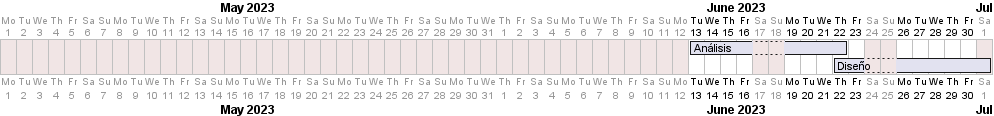
\includegraphics[width=0.01\textwidth]{4-PlanificacionYGestionDelTFG/PlanificacionFinal/gantt/gant2.png}
	\vspace{0.4cm}
	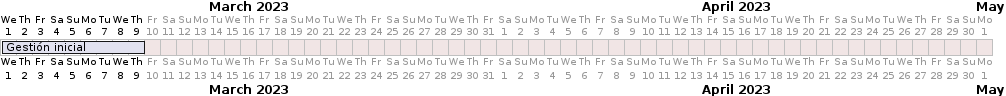
\includegraphics[width=1\textwidth]{4-PlanificacionYGestionDelTFG/PlanificacionFinal/gantt/gant1.png}
	\vspace{0.4cm}
	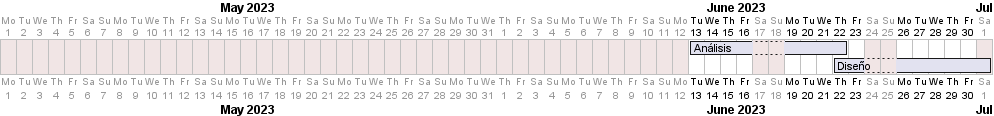
\includegraphics[width=1\textwidth]{4-PlanificacionYGestionDelTFG/PlanificacionFinal/gantt/gant2.png}
	\vspace{0.4cm}
	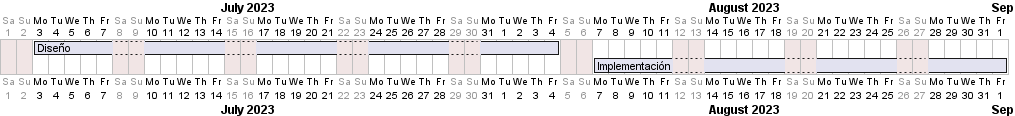
\includegraphics[width=1\textwidth]{4-PlanificacionYGestionDelTFG/PlanificacionFinal/gantt/gant3.png}
	\vspace{0.4cm}
	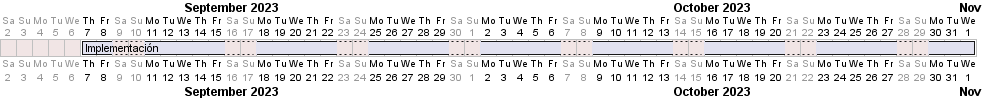
\includegraphics[width=1\textwidth]{4-PlanificacionYGestionDelTFG/PlanificacionFinal/gantt/gant4.png}
	\vspace{0.4cm}
	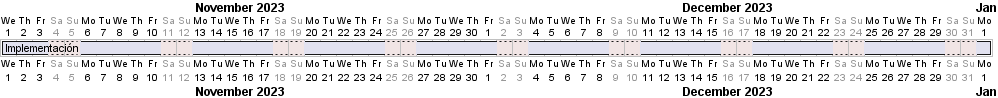
\includegraphics[width=1\textwidth]{4-PlanificacionYGestionDelTFG/PlanificacionFinal/gantt/gant5.png}
	\vspace{0.4cm}
	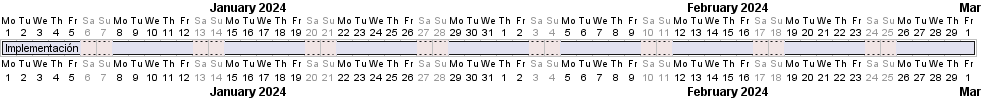
\includegraphics[width=1\textwidth]{4-PlanificacionYGestionDelTFG/PlanificacionFinal/gantt/gant6.png}
	\vspace{0.4cm}
	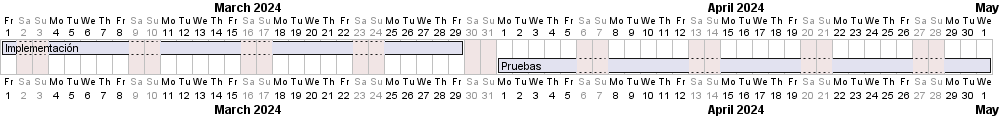
\includegraphics[width=1\textwidth]{4-PlanificacionYGestionDelTFG/PlanificacionFinal/gantt/gant7.png}
	\vspace{0.4cm}
	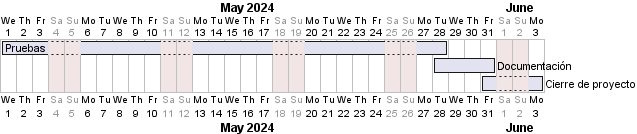
\includegraphics[width=0.6\textwidth]{4-PlanificacionYGestionDelTFG/PlanificacionFinal/gantt/gant8.png}
	\caption{Diagrama de Gantt de la planificación del TFG}
\end{figure}

\begin{figure}[H]
	\centering
	\begin{minipage}{0.45\textwidth}
		\includegraphics[width=0.8\textwidth]{4-PlanificacionYGestionDelTFG/PlanificacionFinal/gantt/gant-gestionInicial.png}
		\caption{Diagrama de Gantt de la fase de gestión inicial}
	\end{minipage}
	\hfill
	\begin{minipage}{0.45\textwidth}
		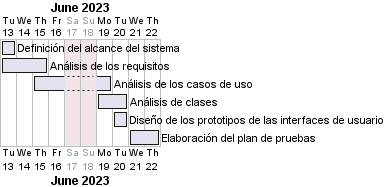
\includegraphics[width=1\textwidth]{4-PlanificacionYGestionDelTFG/PlanificacionFinal/gantt/gant-analisis.png}
		\caption{Diagrama de Gantt de la fase de análisis}
	\end{minipage}
\end{figure}

\begin{figure}[H]
	\includegraphics[width=1\textwidth]{4-PlanificacionYGestionDelTFG/PlanificacionFinal/gantt/gant-diseño.png}
	\caption{Diagrama de Gantt de la fase de diseño}
\end{figure}

\begin{figure}[H]
	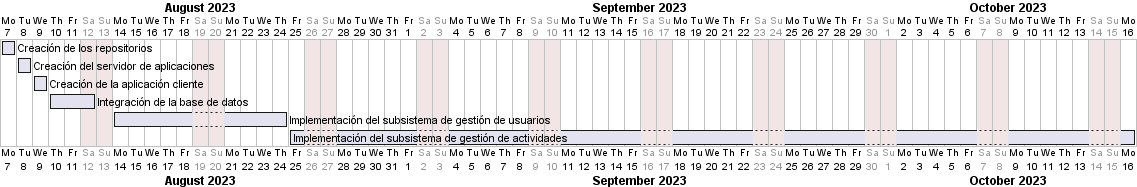
\includegraphics[width=0.01\textwidth]{4-PlanificacionYGestionDelTFG/PlanificacionFinal/gantt/gant-implementacion1.png}
	\vspace{0.4cm}
	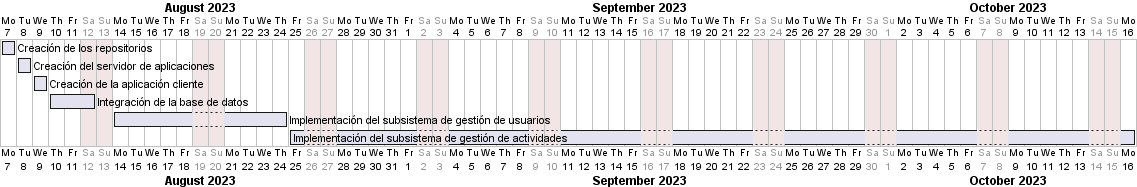
\includegraphics[width=1\textwidth]{4-PlanificacionYGestionDelTFG/PlanificacionFinal/gantt/gant-implementacion1.png}
	\vspace{0.4cm}
	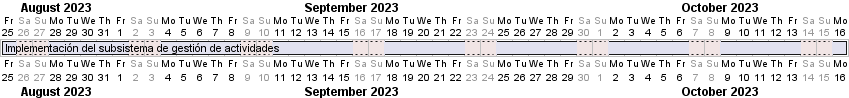
\includegraphics[width=1\textwidth]{4-PlanificacionYGestionDelTFG/PlanificacionFinal/gantt/gant-implementacion2.png}
	\vspace{0.4cm}
	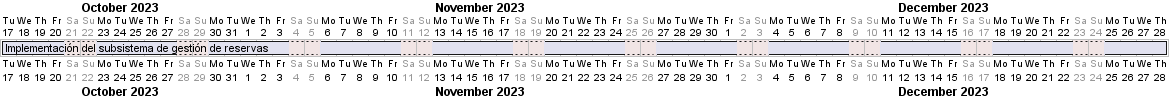
\includegraphics[width=1\textwidth]{4-PlanificacionYGestionDelTFG/PlanificacionFinal/gantt/gant-implementacion3.png}
	\vspace{0.4cm}
	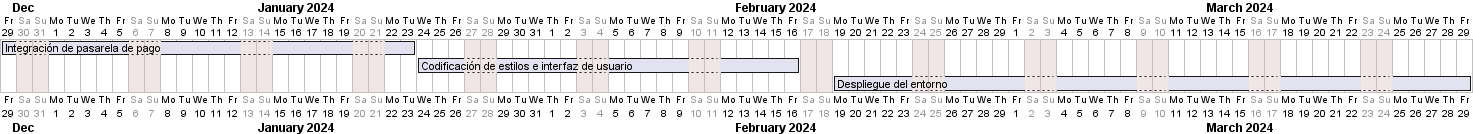
\includegraphics[width=1\textwidth]{4-PlanificacionYGestionDelTFG/PlanificacionFinal/gantt/gant-implementacion4.png}
	\caption{Diagrama de Gantt de la fase de implementación}
\end{figure}

\begin{figure}[H]
	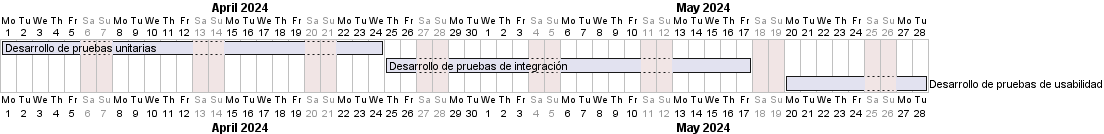
\includegraphics[width=1\textwidth]{4-PlanificacionYGestionDelTFG/PlanificacionFinal/gantt/gant-pruebas.png}
	\caption{Diagrama de Gantt de la fase de pruebas}
\end{figure}

\begin{figure}[H]
	\centering
	\begin{minipage}{0.45\textwidth}
		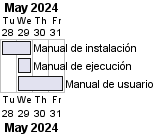
\includegraphics[width=0.5\textwidth]{4-PlanificacionYGestionDelTFG/PlanificacionFinal/gantt/gant-documentacion.png}
		\caption{Diagrama de Gantt de la fase de documentación}
	\end{minipage}
	\hfill
	\begin{minipage}{0.45\textwidth}
		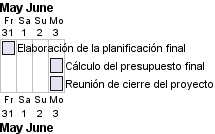
\includegraphics[width=0.6\textwidth]{4-PlanificacionYGestionDelTFG/PlanificacionFinal/gantt/gant-cierre.png}
		\caption{Diagrama de Gantt de la fase de cierre}
	\end{minipage}
\end{figure}

\subsection{Presupuesto Final}
\subsubsection{Presupuesto de costes}
Este es el presupuesto final del proyecto. A continuación, se presenta un desglose detallado de los costes asociados a cada fase del proyecto.
\\[1ex]
Este desglose permite identificar de manera clara y precisa los recursos y costes que ha tenido cada fase.
\begin{planificacion}
	\centering
	\begin{tabular}{ | m{8.5cm} | c | m{2.5cm} |  m{1.5cm} |}
		\hline
		\textbf{Nombre de tarea}                  & \textbf{Duración(horas)} & \textbf{Perfil}         & \textbf{Precio} \\\hline
		Explicación del proyecto                  & 2                        & Director de proyecto    & 67,82€          \\\hline
		Estudio de las alternativas tecnológicas  & 10                       & Consultor de tecnología & 355,50€         \\\hline
		Selección de la arquitectura tecnológica  & 5                        & Arquitecto de software  & 183,25€         \\\hline
		Estudio de viabilidad                     & 15                       & Analista                & 475,80€         \\\hline
		Planificación del proyecto                & 10                       & Director de proyecto    & 339,10€         \\\hline
		Creación de un plan de gestión de riesgos & 8                        & Consultor de tecnología & 284,40€         \\\hline
		Identificación de riesgos                 & 8                        & Consultor de tecnología & 284,40€         \\\hline
	\end{tabular}
	\caption{Presupuesto final de la fase de gestión inicial}
\end{planificacion}

\begin{planificacion}
	\centering
	\begin{tabular}{ | m{8.5cm} | c | m{2.5cm} |  m{1.5cm} |}
		\hline
		\textbf{Nombre de la tarea}                           & \textbf{Duración(horas)} & \textbf{Perfil}    & \textbf{Precio} \\\hline
		Definición del alcance del sistema                    & 5                        & Analista           & 158,60€         \\\hline
		Análisis de los requisitos                            & 15                       & Analista           & 475,80€         \\\hline
		Análisis de los casos de uso                          & 15                       & Analista           & 475,80€         \\\hline
		Análisis de clases                                    & 8                        & Analista           & 253,76€         \\\hline
		Diseño de los prototipos de las interfaces de usuario & 5                        & Diseñador de UX/UI & 128,55€         \\\hline
		Elaboración del plan de pruebas                       & 8                        & Tester             & 131,28€         \\\hline
	\end{tabular}
	\caption{Presupuesto final de la fase de análisis}
\end{planificacion}

\begin{planificacion}
	\centering
	\begin{tabular}{ | m{8.5cm} | c | m{2.5cm} |  m{1.5cm} |}
		\hline
		\textbf{Nombre de la tarea}                      & \textbf{Duración(horas)} & \textbf{Perfil}                & \textbf{Precio} \\\hline
		Diseño de casos de uso reales                    & 15                       & Arquitecto de software         & 549,75€         \\\hline
		Diseño de clases                                 & 10                       & Arquitecto de software         & 366,50€         \\\hline
		Diseño de la arquitectura de módulos del sistema & 8                        & Arquitecto de software         & 293,20€         \\\hline
		Modelado de bases de datos                       & 5                        & Administrador de base de datos & 158,60€         \\\hline
		Diseño de la interfaz de usuario                 & 50                       & Diseñador de UX/UI             & 1285,50€        \\\hline
		Diseño de pruebas                                & 25                       & Tester                         & 410,25€         \\\hline
	\end{tabular}
	\caption{Presupuesto final de la fase de diseño}
\end{planificacion}

\begin{planificacion}
	\centering
	\begin{tabular}{ | m{8.5cm} | c | m{2.5cm} |  m{1.5cm} |}
		\hline
		\textbf{Nombre de la tarea}                             & \textbf{Duración(horas)} & \textbf{Perfil}                & \textbf{Precio} \\\hline
		Creación de los repositorios                            & 2                        & DevOps                         & 43,76€          \\\hline
		Creación del servidor de aplicaciones                   & 2                        & DevOps                         & 43,76€          \\\hline
		Creación de la aplicación cliente                       & 2                        & Desarrollador Full-Stack       & 43,76€          \\\hline
		Integración de la base de datos                         & 5                        & Administrador de base de datos & 158,60€         \\\hline
		Implementación del subsistema de gestión de usuarios    & 20                       & Desarrollador Full-Stack       & 437,60€         \\\hline
		Implementación del subsistema de gestión de actividades & 79                       & Desarrollador Full-Stack       & 1.728,52€       \\\hline
		Implementación del subsistema de gestión de reservas    & 100                      & Desarrollador Full-Stack       & 2188,00€        \\\hline
		Integración de pasarela de pago                         & 50                       & Desarrollador Full-Stack       & 1094,00€        \\\hline
		Codificación de estilos e interfaz de usuario           & 50                       & Diseñador de UX/UI             & 1285,50€        \\\hline
		Despliegue del entorno                                  & 36                       & DevOps                         & 787,68€         \\\hline
	\end{tabular}
	\caption{Presupuesto final de la fase de implementación}
\end{planificacion}

\begin{planificacion}
	\centering
	\begin{tabular}{ | m{8.5cm} | c | m{2.5cm} |  m{1.5cm} |}
		\hline
		\textbf{Nombre de la tarea}          & \textbf{Duración(horas)} & \textbf{Perfil} & \textbf{Precio} \\\hline
		Desarrollo de pruebas unitarias      & 50                       & Tester          & 820,50€         \\\hline
		Desarrollo de pruebas de integración & 40                       & Tester          & 656,40€         \\\hline
		Desarrollo de pruebas de usabilidad  & 15                       & Tester          & 246,15€         \\\hline
	\end{tabular}
	\caption{Presupuesto final de la fase de pruebas}
\end{planificacion}

\begin{planificacion}
	\centering
	\begin{tabular}{ | m{8.5cm} | c | m{2.5cm} |  m{1.5cm} |}
		\hline
		\textbf{Nombre de la tarea} & \textbf{Duración(horas)} & \textbf{Perfil}          & \textbf{Precio} \\\hline
		Manual de instalación       & 2                        & Desarrollador Full-Stack & 43,76€          \\\hline
		Manual de ejecución         & 1                        & Desarrollador Full-Stack & 21,88€          \\\hline
		Manual de usuario           & 8                        & Diseñador de UX/UI       & 205,68€         \\\hline
	\end{tabular}
	\caption{Presupuesto final de la fase de documentación}
\end{planificacion}

\begin{planificacion}
	\centering
	\begin{tabular}{ | m{8.5cm} | c | m{2.5cm} |  m{1.5cm} |}
		\hline
		\textbf{Nombre de la tarea}           & \textbf{Duración(horas)} & \textbf{Perfil}      & \textbf{Precio} \\\hline
		Elaboración de la planificación final & 2                        & Director de proyecto & 67,82€          \\\hline
		Cálculo del presupuesto final         & 2                        & Director de proyecto & 67,82€          \\\hline
		Reunión de cierre del proyecto        & 1                        & Director de proyecto & 33,91€          \\\hline
	\end{tabular}
	\caption{Presupuesto final de la fase de cierre de proyecto}
\end{planificacion}
\subsubsection{Presupuesto total de costes}
En esta sección se presenta una visión global del presupuesto total del proyecto, sumando los costes desglosados por fases y perfiles profesionales.
Como podemos ver en la tabla, el coste total del proyecto asciende a 16652,96€, distribuido en las distintas fases del proyecto. Gracias a ese 20\% de margen de beneficio que se ha añadido al presupuesto inicial, se ha conseguido que el proyecto no se haya excedido del presupuesto inicialmente establecido y además se obtenga un beneficio de 2775,49€.
\begin{planificacion}
	\centering
	\begin{tabular}{ | m{9cm} | c | c |}
		\hline
		\textbf{Fase}      & \textbf{Duración (horas)} & \textbf{Precio}    \\\hline
		Gestión inicial    & 63                        & 2148,87€           \\\hline
		Análisis           & 56                        & 1623,79€           \\\hline
		Diseño             & 113                       & 3063,85€           \\\hline
		Implementación     & 287                       & 7811,18€           \\\hline
		Pruebas            & 105                       & 1723,05€           \\\hline
		Documentación      & 11                        & 271,32€            \\\hline
		Cierre de proyecto & 5                         & 169,55€            \\\hline
		\textbf{Total}     & \textbf{669}              & \textbf{16652,96€} \\\hline
	\end{tabular}
	\caption{Presupuesto de costes total}
\end{planificacion}

\subsection{Informe de lecciones aprendidas}
\begin{itemize}
	\item La comunicación clara y constante con los stakeholders es fundamental para entender correctamente sus necesidades y expectativas
	\item Las estimaciones iniciales a menudo son optimistas y no consideran imprevistos. Habría que incorporar un margen de tiempo adicional para enfrentar posibles imprevistos y revisar las estimaciones con expertos de la materia.
	\item Los riesgos no identificados pueden afectar seriamente al progreso del proyecto.
\end{itemize}
